\chapter{Capa de movimiento para el humanoide}\label{cap:capa_movimiento}

Una vez explicadas las herramientas utilizadas en el capítulo anterior, en este se explicará el proyecto como tal, desglosando adecuadamente cada una de las partes involucradas en él.

\section{Preparación del modelo simulado} \label{sec:prep_modelo}

Cómo se mencionó en el capítulo \ref{cap:herramientas}, el modelo utilizado fue extraído de la librería abierta de Gazebo.
Sin embargo, este modelo no era suficiente para poder desarrollar todo el proyecto directamente y fue necesario prepararlo y adaptarlo.

\subsection{Compatibilidad del modelo con ROS2}

Lo primero que se hizo para poder usar el modelo fue preparar los \textit{topics} de ROS2 necesarios para publicar posiciones en sus articulaciones y así hacer el modelo compatible con este middleware, ya que como se aprecia en la \autoref{fig:topics_independientes}, tenía los \textit{topics} preparados para Gazebo, y no para ROS. Esto es porque en la versión de Gazebo de 2018, Gazebo Ignition/Gazebo Sim, el simulador se rediseñó desde cero con la idea de ser más independiente de ROS, para que así los usuarios no estuvieran obligados a utilizar dicho middleware para lanzar simulaciones. 

\begin{figure}[H]
  \centering
  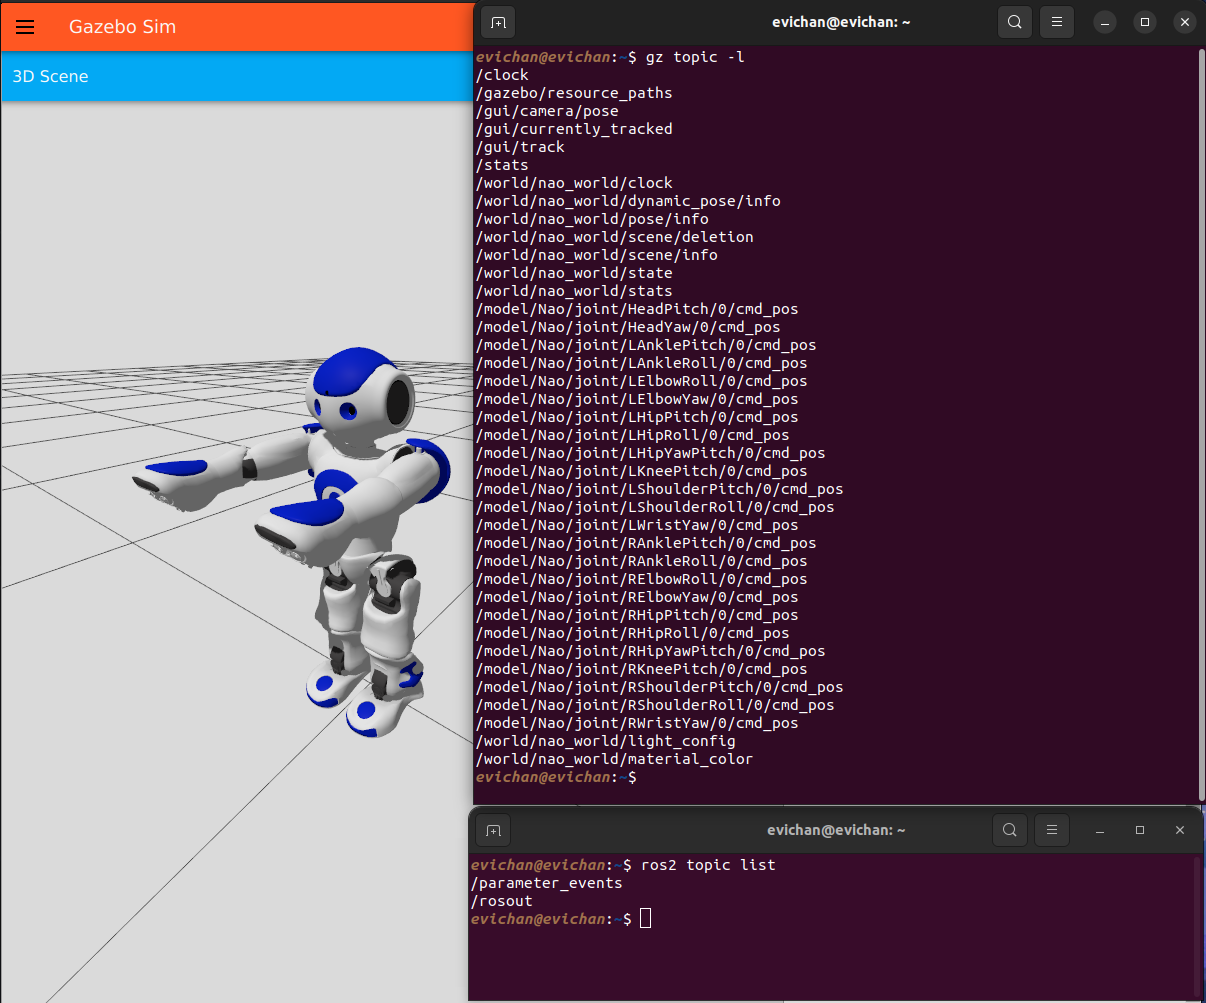
\includegraphics[width=1\textwidth]{figures/cap_4/topics_gazebo.png}
  \caption{\textit{topics} sólo accesibles desde Gazebo y no desde ROS2}
  \label{fig:topics_independientes}
\end{figure}

La solución para este pequeño problema es utilizar un puente que conecta los \textit{topics} de Gazebo con los \textit{topics} de ROS2, disponible en el paquete \textit{ros\_gz\_bridge}\footnote{\url{https://github.com/gazebosim/ros_gz/tree/ros2/ros_gz_bridge}}, que se encarga de que los \textit{topics} de Gazebo sean también visibles al ejecutar el comando \texttt{ros2 topic list}, y no solo al ejecutar \texttt{gz topic -l}, permitiendo trabajar con ellos desde ROS2.

Para aplicar este puente, se instala el paquete con \texttt{sudo apt install ros-humble-ros-gz-bridge}. Después, es necesario crear el paquete de ROS que será usado para alojar todos los programas que se iban a lanzar y, además de eso, se debe crear un \textit{launcher.py}, encargado de lanzar la simulación y todos los puentes necesarios para los \textit{topics} de NAO accesibles en Gazebo (todos aquellos que siguen la estructura \textit{/model/NAO/joint/..../0/cmd\_pos}).

Sin embargo, los nombres de los \textit{topics} de Gazebo contienen el número 0 en sus nombres, cosa incompatible con los \textit{topics} de ROS2. Por lo que el primer cambio que se tuvo que hacer al modelo fue cambiar el nombre de todos los \textit{topics} relacionados con el movimiento del robot, para así eliminar este número 0. 

Para ello, en el fichero SDF del robot, primero se tenía que localizar dónde se alojaban esos \textit{topics}, ya que el modelo no disponía de una etiqueta \textit{topic} o similar. Esto es porque que para poder crear estos \textit{topics}, Gazebo utiliza \textit{plugins}\footnote{\url{https://gazebosim.org/libs/plugin/}}. 

Estos plugins son fragmentos de código (generalmente en C++) que se cargan en tiempo de ejecución dentro del simulador para extender o modificar su comportamiento, permitiendo agregar funcionalidades personalizadas a los modelos o mundos.

En el caso de los \textit{topics}, el \textit{plugin} responsable se especifica debajo de cada \textit{joint} (articulación) en el archivo SDF del robot NAO de la forma mostrada en el \autoref{lst:plugin_original}:

\begin{lstlisting}[language=XML, caption={Inclusión del plugin en el modelo}, label={lst:plugin_original}, numbers=left, backgroundcolor=\color{gray!10}]    
<plugin
  filename="ignition-gazebo-joint-position-controller-system"
  name="ignition::gazebo::systems::JointPositionController">
  <joint_name>HeadYaw</joint_name>
  <p_gain>10</p_gain>
  <i_gain>0.1</i_gain>
  <d_gain>0.01</d_gain>
  <i_max>1</i_max>
  <i_min>-1</i_min>
  <cmd_max>1000</cmd_max>
  <cmd_min>-1000</cmd_min>
</plugin>
\end{lstlisting}

En dicho código se especifican todas las condiciones necesarias para que la articulación se comporte como un motor real, incluyendo incluso un controlador PID, con sus ganancias p\_gain, i\_gain y d\_gain. Lo importante aquí es que el nombre del \textit{topic} no está definido, y es por eso por lo que se recoge el nombre por defecto, el que incluye el número cero en su nombre.

Para cambiar esto, sólo es necesario añadir la línea \texttt{<topic>nombre\_deseado</topic>} en cualquier lugar de la definición del \textit{plugin}. Una vez hecho esto para todos los \textit{topics}, quedaron como se muestra en la \autoref{fig:topics_independientes_cambiados}:

\begin{figure}[H]
  \centering
  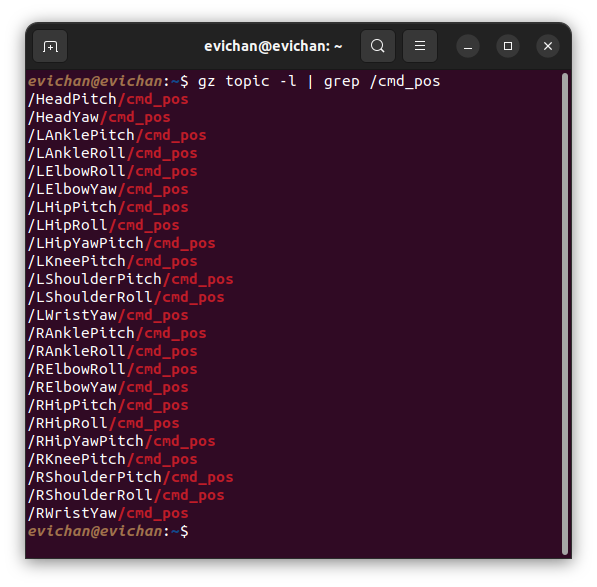
\includegraphics[width=1\textwidth]{figures/cap_4/topics_gazebo_cambiados.png}
  \caption{\textit{topics} corregidos para poder hacer el puente}
  \label{fig:topics_independientes_cambiados}
\end{figure}

Ahora, los \textit{topics} están en el formato correcto para ROS2, por lo que el puente es realizable.

Para crear este puente es necesario incluir en el lanzador del simulador los comandos necesarios para ello. Esto se hace añadiendo las líneas de código que se muestran en el \autoref{lst:estructura_bridge} al \textit{launcher.py} (\cite{tutorial_bridge}):

\begin{lstlisting}[language=Python, caption={Estructura de un \texttt{gz\_bridge}}, label={lst:estructura_bridge}, numbers=left, backgroundcolor=\color{gray!10}]    
gz_bridge_1 = Node(
    package="ros_gz_bridge",
    executable="parameter_bridge",
    name="gz_bridge",
    arguments=[
        "nombre_topic" + "direccion_del_puenteTipo_de_mensaje_ros" + "direccion_del_puenteTipo_de_mensaje_gazebo"
    ],
    output="screen",
)
\end{lstlisting}

Para la dirección del puente, hay que escribir uno de los siguientes símbolos:

\begin{itemize}
  \item \texttt{[:} Puente unidireccional desde Gazebo a ROS. Este puente sólo permite que ROS se suscriba a los \textit{topics}, pero no puede publicar en ellos.
  \item \texttt{]:} Puente unidireccional desde ROS a Gazebo. Este es el caso contrario al anterior, ROS puede publicar, pero no suscribirse.
  \item \texttt{@:} Puente bidireccional. Este puente permite mensajes en ambas direcciones, por lo que ROS puede publicar o suscribirse sin problemas.
\end{itemize}

En este caso, se ha utilizado un puente bidireccional en todos los \textit{topics}, para poder publicar mensajes y suscribirnos a ellos si es necesario.

Para los tipos de mensajes utilizables, es necesario consultar la compatibilidad entre ellos en la tabla\footnote{\url{https://github.com/gazebosim/ros_gz/tree/ros2/ros_gz_bridge/README.md}} dada en el repositorio oficial del paquete \textit{ros\_gz\_bridge}, no sin antes consultar qué tipo tienen los \textit{topics} de Gazebo utilizando el comando \texttt{gz topic -i -t nombre\_del\_topic}.

Una vez definido el tipo de mensajes a utilizar (en el caso de este proyecto, \textit{std\_msgs/msg/Float64 para} ROS y \textit{gz.msgs.Double} para Gazebo), se desarrolló de forma sencilla el \textit{launcher} del robot con los \textit{topics} de sus articulaciones compatibles con ROS2. Para ello, se siguió el esquema mostrado en la \autoref{lst:estructura_bridge} y se usaron los componentes necesarios para crear un lanzador adecuado. Un fragmento de dicho \textit{launcher} se ve en el \autoref{lst:launcher}.

\begin{lstlisting}[language=Python, caption={Ejemplo de launcher para simulación}, label={lst:launcher}, numbers=left, backgroundcolor=\color{gray!10}]    
#!/usr/bin/env python3
# Importaciones necesarias
def generate_launch_description():
    set_gazebo_version = SetEnvironmentVariable(
        name="GAZEBO_VERSION", value="8.9"
    )
    # Para poder lanzar el mundo
    world_file = PathJoinSubstitution(['/home/evichan/Desktop/2024-tfg-eva-fernandez/GreenNao/greennao/worlds/greenhouse_world', 'greenhouse_world.sdf'])
    declare_world_arg = DeclareLaunchArgument(
        "world", default_value=world_file, description="SDF world file"
    )
    # Para lanzar simulacion de gazebo
    gz_sim = IncludeLaunchDescription(
        PythonLaunchDescriptionSource(
            PathJoinSubstitution(
                [
                get_package_share_directory("ros_gz_sim"),
                    "launch",
                    "gz_sim.launch.py",
                ]
            )
        ),
        launch_arguments={"gz_args": world_file}.items(),
    )
    # Ros bridges para controlar articulaciones de NAO van aqui, uno por grado de libertad
    [...]
    return LaunchDescription(
        [
            declare_world_arg,
            set_gazebo_version,
            SetParameter(name="use_sim_time", value=True),
            gz_sim,
            gz_bridge_1,
            [...] # resto de bridges
        ]
    )
\end{lstlisting}

Una vez ejecutado este \textit{launcher}, además de ver el mundo creado y la simulación completa, podemos ver en la terminal cómo ahora los \textit{topics} se comparten entre ROS2 y Gazebo. Un ejemplo de esto se muestra en la \autoref{fig:topics_ros}.

\begin{figure}[H]
  \centering
  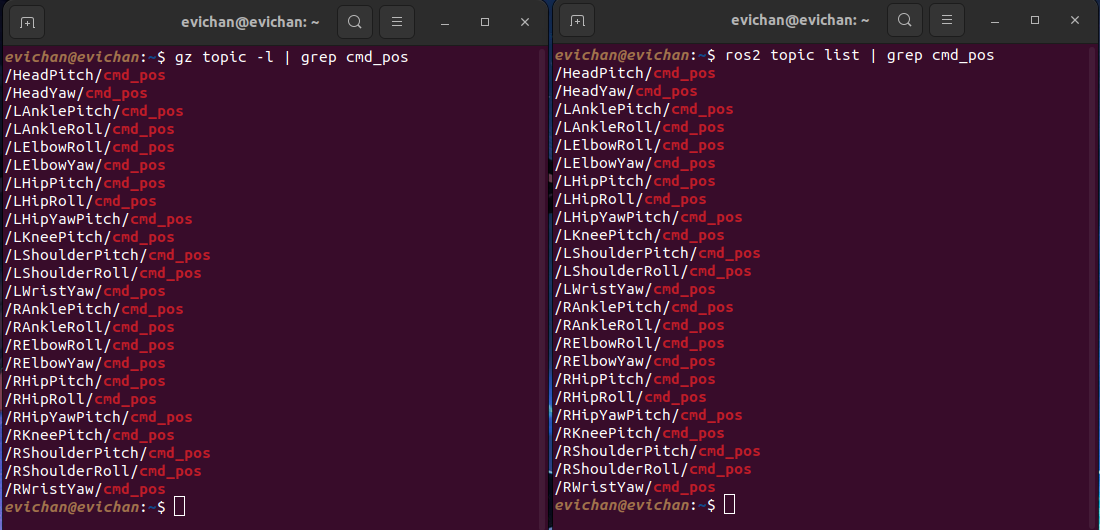
\includegraphics[width=1\textwidth]{figures/cap_4/topics_ros.png}
  \caption{\textit{topics} accesibles desde ROS2 y Gazebo}
  \label{fig:topics_ros}
\end{figure}

\subsection{Adición de sensores}

No sólo fue necesario hacer el modelo compatible con ROS2, sino que también fue  necesario
enriquecer un poco al robot dotándole de sensores, ya que el modelo de Gazebo no los ofrecía. Se optó por añadir una cámara y un sensor IMU para que fueran usables en el futuro, además de que son sensores muy utilizados en robótica en general.

\subsubsection{Cámara}
Para añadir una cámara al robot y dotarle de visión, fue necesario insertarle al modelo los campos necesarios para que tuviera una cámara completamente funcional y usable con ROS2, así que, para ello, se añadieron los elementos mostrados en el \autoref{lst:camara_modelo} al SDF del modelo.

\begin{lstlisting}[language=XML, caption={Adición de la cámara al modelo}, label={lst:camara_modelo}, numbers=left, backgroundcolor=\color{gray!10}]   
# Definicion del joint necesario para anclar la camara al torso del robot
[...]
<link name="camera_rgb_frame">
  # Definicion de masa e inercia para en sensor
  [...]
  <sensor name="camera" type="camera">
    <always_on>true</always_on>
    <visualize>true</visualize>
    <update_rate>30</update_rate>
    <topic>NAO/camera/image_raw</topic>
    <gz_frame_id>camera_rgb_frame</gz_frame_id>
    <camera name="intel_realsense_r200">
      <camera_info_topic>NAO/camera/camera_info</camera_info_topic>
      <horizontal_fov>1.02974</horizontal_fov>
      <image>
        <width>1920</width>
        <height>1080</height>
        <format>R8G8B8</format>
      </image>
      <clip>
        <near>0.02</near>
        <far>300</far>
      </clip>
      <noise>
        <type>gaussian</type>
        <mean>0.0</mean>
        <stddev>0.007</stddev>
      </noise>
    </camera> 
  </sensor>
</link>
<plugin filename="gz-sim-sensors-system" name="gz::sim::systems::Sensors">
    <render_engine>ogre2</render_engine>
</plugin>
\end{lstlisting}

\subsubsection{Sensor IMU}
Para que el robot pudiera localizarse utilizando una IMU, fue necesario añadir los siguientes campos al modelo dentro del \textit{link} del torso:

\begin{lstlisting}[language=XML, caption={Adición del sensor IMU al modelo}, label={lst:imu_modelo}, numbers=left, backgroundcolor=\color{gray!10}]    
<sensor name="imu_sensor" type="imu">
    <pose>0 0 0 0 0 0</pose>
    <always_on>true</always_on>
    <update_rate>50</update_rate>
    <visualize>true</visualize>
    <topic>NAO/imu_sensor</topic>
    <imu>
    <angular_velocity>
        <noise>
        <type>gaussian</type>
        <mean>0.0</mean>
        <stddev>0.01</stddev>
        </noise>
    </angular_velocity>
    <linear_acceleration>
        <noise>
        <type>gaussian</type>
        <mean>0.0</mean>
        <stddev>0.01</stddev>
        </noise>
    </linear_acceleration>
    </imu>
</sensor>       
</link>
<plugin filename="gz-sim-imu-system" name="gz::sim::systems::Imu">
    <topic>NAO/imu_sensor</topic>
</plugin> 
\end{lstlisting}

Después de añadir estos sensores al SDF del modelo, se añadieron también los puentes necesarios al \textit{launcher} para que ROS pudiera acceder a sus lecturas, de la misma forma vista anteriormente en el \autoref{lst:launcher}.

Una vez los sensores fueron añadidos correctamente, los \textit{topics} finales del robot eran los siguientes:

\begin{figure}[H]
  \centering
  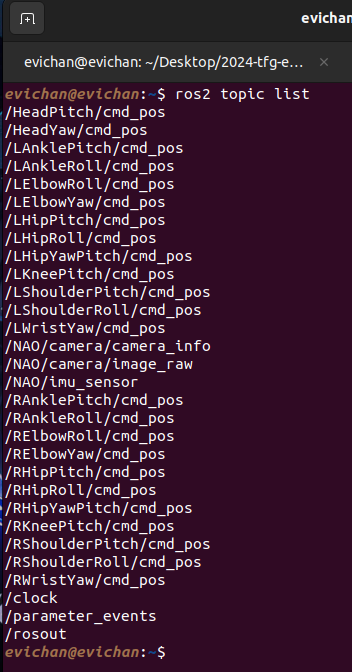
\includegraphics[width=0.5\textwidth]{figures/cap_4/topics_completos.png}
  \caption{\textit{topics} finales del robot}
  \label{fig:topics_completos}
\end{figure}

\subsection{Estabilidad estática}

Un problema que tienen los robots humanoides, como se comentaba en el capítulo \ref{cap:introduccion}, es que tienen que ser estables tanto dinámica cómo estáticamente, y el NAO no es una excepción.

Cuando se probó el robot en el mundo por primera vez, éste caía de boca al suelo, cosa que indicaba que el modelo no era estáticamente estable.

Para dotarle de esta estabilidad, se compensó el peso del humanoide con las posiciones iniciales de sus articulaciones y su posición inicial, a base prueba y error.

Cambiar la posición inicial no tiene ningún misterio, ya que simplemente es cambiar el campo \textit{pose} que está al incio del modelo. Sin embargo, las posiciones iniciales de las articulaciones tuvieron más complicación. Para asignarlas, fue necesario añadir los campos \texttt{<initial\_position>} y \texttt{<use\_velocity\_commands>true</use\_velocity\_commands>}, seguido de los campos \texttt{cmd\_max} y \texttt{cmd\_min} al plugin de las articulaciones para que la velocidad no fuera demasiado brusca para el movimiento y la articulación se moviera correctamente a la posición deseada al comienzo de la simulación. Se adjunta a continuación un ejemplo de estos cambios (\autoref{lst:ejemplo_posicion_inicial}), y un vídeo\footnote{\url{https://youtu.be/u6OsTDhBnuk}} del resultado final de este cambio.  

\begin{lstlisting}[language=XML, caption={Ejemplo de configuración de posición inicial de una articulación}, label={lst:ejemplo_posicion_inicial}, numbers=left, backgroundcolor=\color{gray!10}]    
<plugin filename="ignition-gazebo-joint-position-controller-system" name="ignition::gazebo::systems::JointPositionController">
    [...]
    <use_velocity_commands>true</use_velocity_commands>
    <cmd_max>2.0</cmd_max>
    <cmd_min>-2.0</cmd_min>
    [...]
    <initial_position>1.39626</initial_position>
</plugin>
\end{lstlisting}

Por tanto, para lograr esta estabilidad estática, el robot debe comenzar con las siguientes posiciones:

\begin{itemize}
  \item Posición inicial del robot: x=0 y=0 z=0.5 rx=0 ry=0.240818894505798 rx=0
  \item /HeadPitch/cmd\_pos: 0
  \item /HeadYaw/cmd\_pos: 0
  \item /LAnklePitch/cmd\_pos: -0.479
  \item /LAnkleRoll/cmd\_pos: 0
  \item /LElbowRoll/cmd\_pos: -1.0472
  \item /LElbowYaw/cmd\_pos: -1.39626
  \item /LHipPitch/cmd\_pos: -0.179
  \item /LHipRoll/cmd\_pos: 0
  \item /LHipYawPitch/cmd\_pos: 0
  \item /LKneePitch/cmd\_pos: 0.698132
  \item /LShoulderPitch/cmd\_pos: 1.39626
  \item /LShoulderRoll/cmd\_pos: 0.198132
  \item /LWristYaw/cmd\_pos: -0.192
  \item /RAnklePitch/cmd\_pos: -0.479
  \item /RAnkleRoll/cmd\_pos: 0
  \item /RElbowRoll/cmd\_pos: 1.0472
  \item /RElbowYaw/cmd\_pos: 1.39626
  \item /RHipPitch/cmd\_pos: -0.179
  \item /RHipRoll/cmd\_pos: 0
  \item /RHipYawPitch/cmd\_pos: 0
  \item /RKneePitch/cmd\_pos: 0.698132
  \item /RShoulderPitch/cmd\_pos: 1.39626
  \item /RShoulderRoll/cmd\_pos: -0.198132
  \item /RWristYaw/cmd\_pos: 0.192
\end{itemize}

También fue necesario editar el peso de ambos pies. Esto porque el robot tenía más peso en el tren superior que en el inferior y esto le impedía levantarse, así que se sumó 1 kilogramo de peso a cada pie y se modificaron sus matrices de inercia para adaptarlos correctamente a su nueva masa.

\subsection{Retoque estético}

Cómo último preparativo del modelo, se editó su textura para que fuera de color verde, así se lograría dar un poco de identidad al modelo y, de cara a la aplicación final en un invernadero, que fuera más vistoso.

El resultado de este retoque se puede ver en la \autoref{fig:nao_retocado}.

\begin{figure}[H]
  \centering
  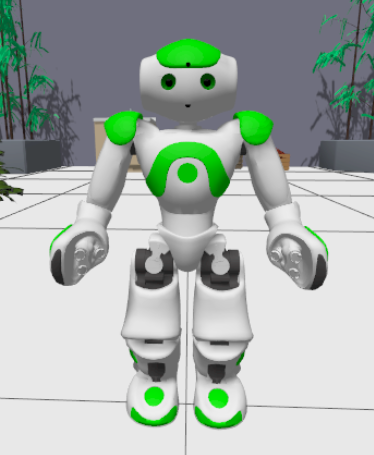
\includegraphics[width=0.5\textwidth]{figures/cap_4/GreenNao.png}
  \caption{Nao retocado estéticamente}
  \label{fig:nao_retocado}
\end{figure}

Una vez terminadas estas modificaciones, el modelo estaba completamente preparado, ya era posible su programación, y por ende el desarrollo del resto del proyecto como tal.

\section{Editor gráfico e intérprete de movimientos}

El primer elemento clave de este proyecto es el editor de movimientos, una herramienta capaz de crear patrones fijos de movimiento para coordinar las articulaciones de NAO de forma cómoda.

Una vez creados estos patrones, para materializarlos en movimiento, es necesario crear un intérprete que permita a NAO replicar dichos patrones, también de forma cómoda. Es por esto que editor e intérprete van de la mano y se describen a continuación. También se adjunta en la \autoref{fig:esquema_editor_interprete} un esquema para ilustrar de forma adecuada este concepto.

\begin{figure}[H]
  \centering
  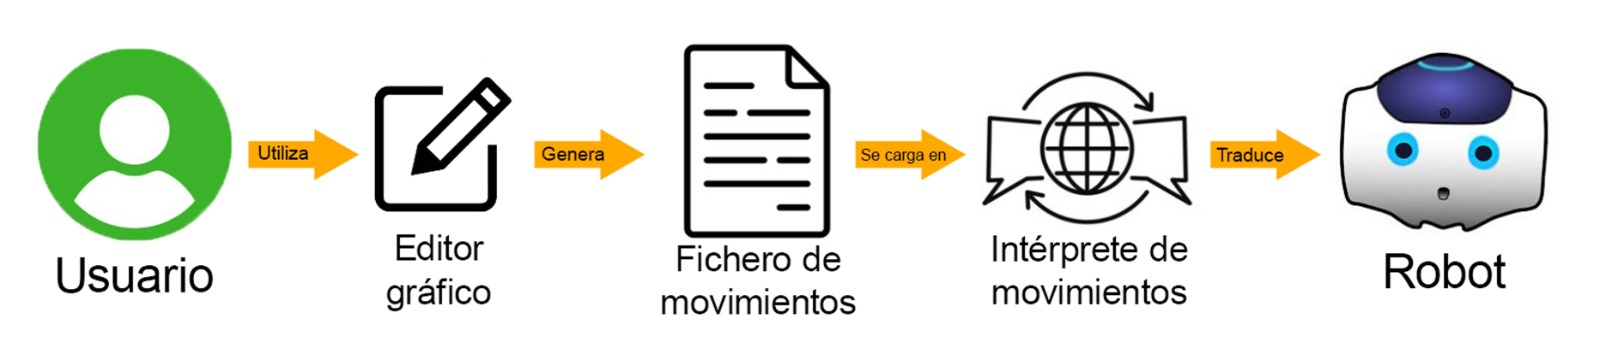
\includegraphics[width=1.05\textwidth]{figures/cap_4/esquema_ed_in.jpeg}
  \caption{Esquema del funcionamiento del editor y el intérprete}
  \label{fig:esquema_editor_interprete}
\end{figure}

\subsection{Editor gráfico} \label{subsec:editor}

Este editor consiste en un programa que permite al usuario crear patrones de movimiento para que posteriormente sean procesados por el intérprete y a su vez replicados por el robot. Está basado en \textit{KME} (\cite{paper_1},\cite{paper_2}), un editor de movimientos basado en fotogramas clave (\textit{keyframes}). Permite al usuario crear secuencias de posiciones para cada articulación del robot en momentos específicos del tiempo. Es especialmente útil para programar movimientos complejos y que requieren de la coordinación de varios actuadores simultáneamente, como saludar o tomar una pose concreta, siendo estos patrones siempre fijos y no modificables a la hora de interpretarse.

El programa se ha desarrollado en Pyhton, y utiliza el simulador Pybullet\footnote{\url{https://Pybullet.org/wordpress/index.php/forum-2/}} para poder ofrecer al usuario una visión directa del NAO y sus movimientos a la hora de crear el patrón.

Para que todo funcionase correctamente en Pybullet, era necesario tener disponible al modelo 3D de NAO, para cumplir la parte de la visualización en tiempo real de los movimientos.

Sin embargo, el formato SDF del modelo que se preparó no es compatible con Pybullet, siendo el formato requerido URDF. Por suerte, se encontró un modelo de NAO en URDF disponible para descargar en un repositorio público de github\footnote{\url{https://github.com/ros-naoqi/nao_robot/blob/master/nao_description/urdf/naoV40_generated_urdf/nao.urdf}}. También fue necesario modificar este URDF para que fuera lo más igual posible al modelo en SDF, esto es, ponerle las posiciones iniciales de las articulaciones (cosa que se hace directamente en el código del editor), editar los pesos de los pies para que fueran iguales a los del SDF, ajustar los límites de las articulaciones, etc. 

La aplicación del editor gráfico es capaz de conectarse a los \textit{joints} de NAO gracias a Pybullet, que dispone de una API específica para hacerlo, por lo que es necesario tener en cuenta todos los \textit{topics} (de las articulaciones) que se iban a manejar y qué movimientos y grados de libertad tenemos disponibles. Para eso es muy útil el esquema mostrado en la \autoref{fig:esquema_joints}:

\begin{figure}[H]
  \centering
  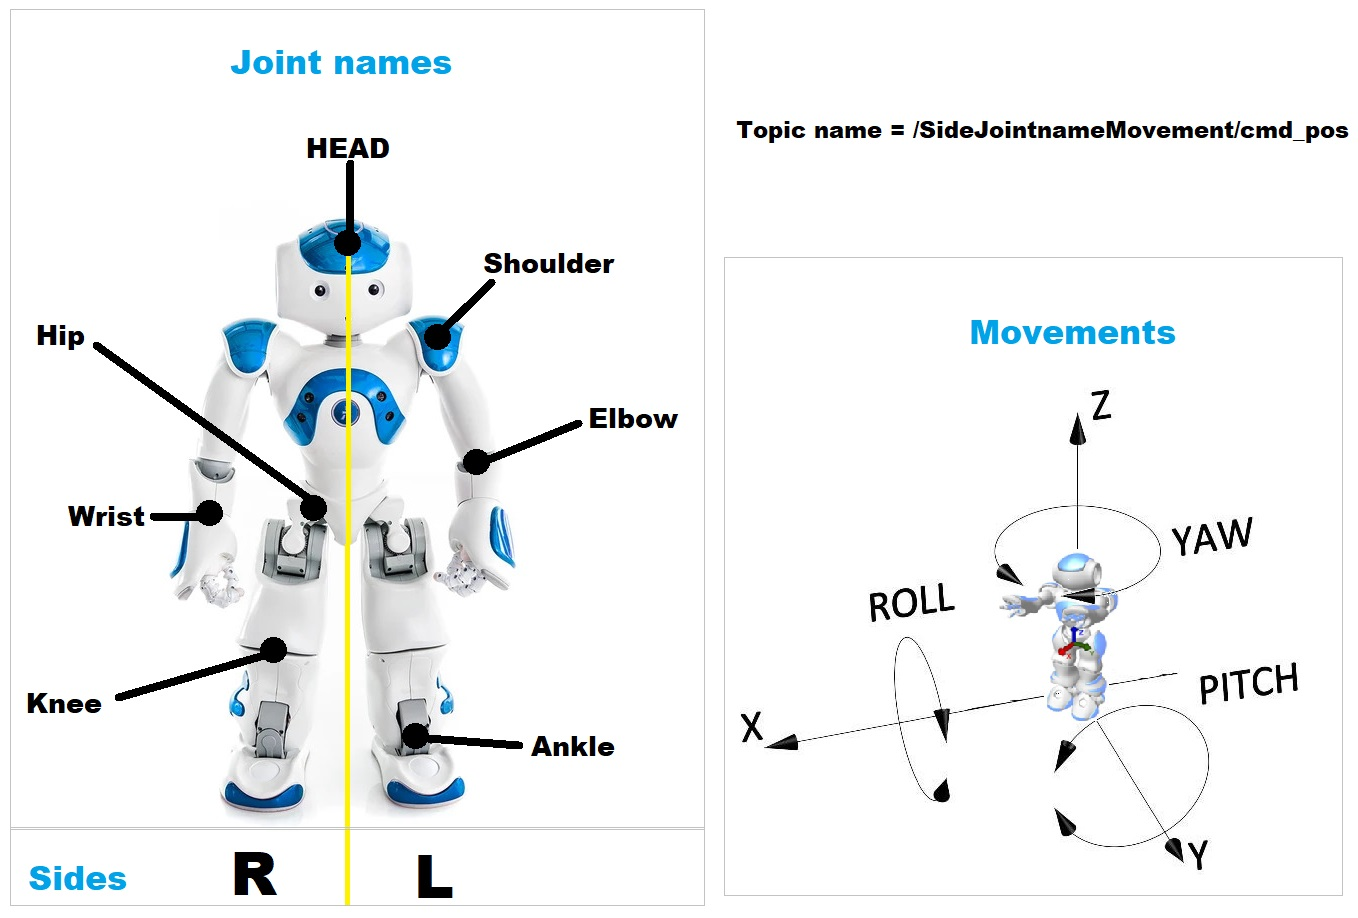
\includegraphics[width=1\textwidth]{figures/cap_4/esquema_joints_NAO.jpeg}
  \caption{Esquema de \textit{topics} y articulaciones de NAO}
  \label{fig:esquema_joints}
\end{figure}

Cómo se puede ver, este robot ofrece mucha variedad de movimientos, con un total de 24 grados de libertad.

Para controlar cada uno de ellos en Pybullet de forma cómoda se ofrece una interfaz gráfica con barras deslizantes o \textit{sliders} para que el manejo sea más visual y fácil de abarcar, esto es porque las articulaciones tienen un límite y no todas las posiciones son válidas. Con estas barras el usuario puede ver fácilmente dichos límites.

Este sistema de \textit{sliders} lo ofrece Pybullet de forma cómoda, simplemente escribiendo lo mostrado en el \autoref{lst:ejemplo_slider} en el código del editor:

\begin{lstlisting}[language=Python, caption={Ejemplo de adicición de sliders al editor}, label={lst:ejemplo_slider}, numbers=left, 
backgroundcolor=\color{gray!10}]    

# Preparar el slider
joint_slider = p.addUserDebugParameter("nombre del joint", minimo, maximo, posicion inicial)

# Dentro del bucle principal (omitido ahora) Lectura del slider
joint_value = p.readUserDebugParameter(joint_slider)

# Ejecucion del movimiento en el modelo
p.setJointMotorControl2(model,1, p.POSITION_CONTROL, targetPosition=joint_value, maxVelocity=2)
\end{lstlisting}

Con esto para cada una de las articulaciones, el usuario es capaz de controlar íntegramente a NAO, aún sin posibilidad de guardar los movimientos deseados.

Para esto se han utilizado ficheros JSON, de modo que se han añadido 2 \textit{sliders} adicionales, uno para indicar el tiempo en el que se desea adoptar esa posición (tiempo del fotograma), y otro más que indica al programa que se quiere guardar el patrón, el cual, cuando cambia de posición, guarda automáticamente el fichero y avisa al usuario.

Un ejemplo del formato que tienen estos ficheros JSON se muestra en el \autoref{lst:ejemplo_json}.

\begin{lstlisting}[language=, caption={Ejemplo de JSON}, label={lst:ejemplo_json}, numbers=left, 
backgroundcolor=\color{gray!10}]    
[
    {
        "tiempo": 1, # marca de tiempo
        "articulaciones": [
            {
                "articulacion": "HeadYaw",
                "posicion": 2.0901734911206137e-08
            },
            {
                "articulacion": "HeadPitch",
                "posicion": 1.8516262613600133e-08
            },
            {
                "articulacion": "LHipYawPitch",
                "posicion": -1.8007272938374389e-09
            },
            {
                "articulacion": "LHipRoll",
                "posicion": -6.113291356754397e-09
            },
            [...] # resto de articulaciones
        ]
    }
]
\end{lstlisting}

Se adjunta un enlace a un vídeo\footnote{\url{https://youtu.be/jkSdVGjrn4s}} demostrativo del funcionamiento de este programa. Cabe destacar que se deja caer al robot al inicio del programa para que el usuario vea que efectivamente hay movimientos y físicas realistas involucrados en él. Se muestra una imagen de este editor en la \autoref{fig:editor_grafico}.

\begin{figure}[H]
  \centering
  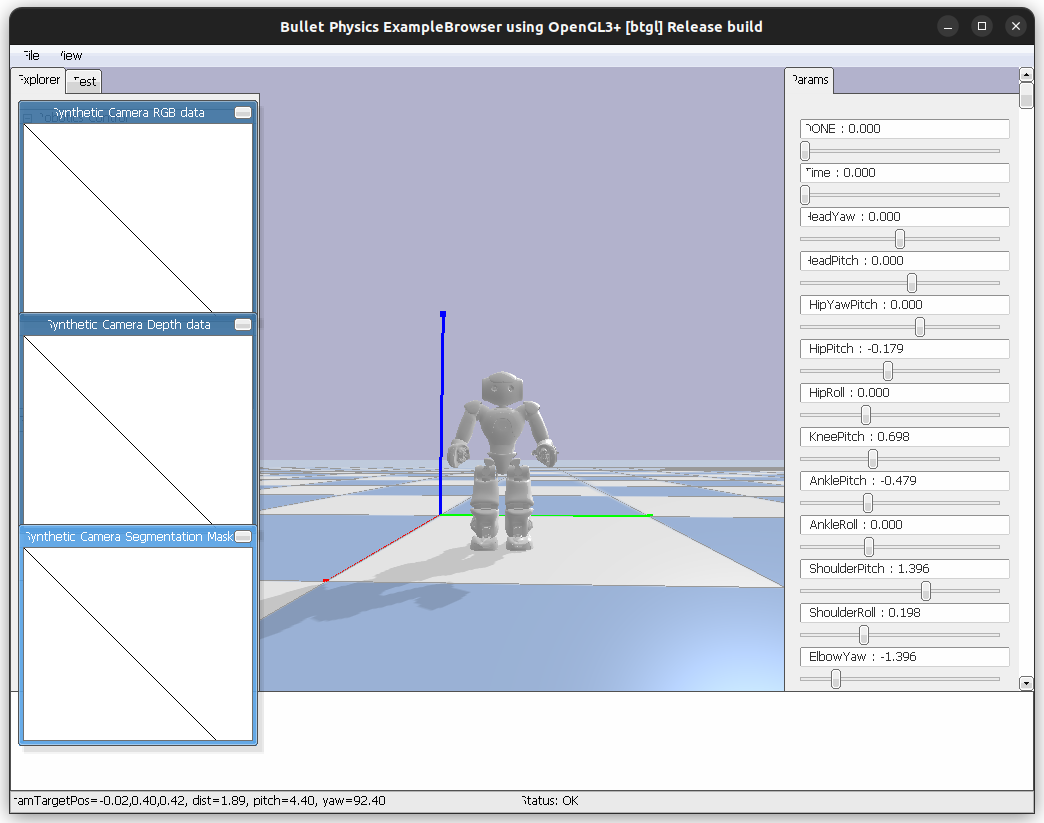
\includegraphics[width=1\textwidth]{figures/cap_4/editor.png}
  \caption{Editor gráfico de movimientos}
  \label{fig:editor_grafico}
\end{figure}

\subsection{Intérprete de movimientos} \label{subsec:interprete}

El editor por si solo no resulta muy útil sin que el robot NAO simulado replique los patrones de movimiento creados. Es por eso por lo que existe el intérprete de movimientos. Este programa consiste en un nodo ROS2 programado en Python que lee los datos del fichero JSON que se le indica por argumento, y se encarga de hacer las publicaciones a los \textit{topics} necesarios en el momento adecuado (replica cada fotograma en la marca de tiempo especificada).

También el usuario podría querer utilizar otros formatos para ficheros que almacenan los movimientos concretos, como el .motion, ofrecido por el simulador Webots\footnote{\url{https://cyberbotics.com/}}. Además, muchos patrones de movimiento ofrecidos en esta aplicación se han conseguido a partir de los ficheros de este simulador, cosa que se explicará con detalle en la seguiente sección. Como Python no ofrece soporte para leer ese tipo de ficheros directamente, se optó por adpatarlos a formato CSV y después añadir también al nodo intérprete la posibilidad de leer este tipo de ficheros.

Para hacer este nodo, se ha utilizado una calidad de servicio como la que se muestra en el \autoref{lst:calidad_de_servicio} para evitar la fatiga a la hora de publicar varios mensajes, ya que estaremos casi constantemente publicando mensajes en cada articulación.

\begin{lstlisting}[language=Python, caption={Calidad de servicio utilizada para publicación de mensajes}, label={lst:calidad_de_servicio}, numbers=left, backgroundcolor=\color{gray!10}]    
qos_profile = QoSProfile(
            reliability=ReliabilityPolicy.RELIABLE,
            history=HistoryPolicy.KEEP_ALL,
            depth=100
)
\end{lstlisting}
 
A continuación, se adjunta un vídeo\footnote{\url{https://youtu.be/sLobRujULKE}} demostrativo de este intérprete de movimientos en funcionamiento para ejecutar movimientos.

Este intérprete se creó inicialmente como un programa aislado, un nodo ROS independiente, sin embargo, se refactorizó  como una función dentro de la librería que se ha desarrollado, de modo que cualquier aplicación con el humanoide pueda utilizarlo para materializar la locomoción y los movimientos del robot. 

\section{Librería de movimientos} \label{sec:librería}

En cuanto a la librería desarrollada, cuyo nombre es \textit{CoordmovesLib.py}, se encarga de que el uso de ROS2 sea parcialmente transparente para el usuario, ya que su instalación y uso básico (creación de un paquete para utilizarla, compilarlo, etc) sigue siendo necesario.

Para lograr este encapsulamiento, la biblioteca debe incluir los nodos necesarios (clases de Python responsables de publicar las posiciones de las articulaciones) y una función que los active, la cual será invocada por el usuario.

La activación de estos nodos requiere el uso de rclpy\footnote{\url{https://docs.ros.org/en/rolling/p/rclpy/}}, que proporciona la API oficial de Python para interactuar con ROS 2.

Un ejemplo de cómo han de crearse estas clases para que los nodos funcionen correctamente se muestra en el \autoref{lst:funcion_rclpy}.

\begin{lstlisting}[language=Python, caption={Ejemplo de función que invoca un nodo ROS2}, label={lst:funcion_rclpy}, numbers=left, backgroundcolor=\color{gray!10}]    
def Interpreter(file_name: str, printable=True):
    rclpy.init()
    node = Interpreter_class(file_name, printable)
    
    try:
        rclpy.spin_once(node, timeout_sec=2)
    
    finally:
      node.destroy_node()
      rclpy.shutdown()
\end{lstlisting}

Hay 3 tipos de estas funciones, las que sirven para llamar a métodos cuya tarea es replicar patrones fijos creados con el intérprete; las que sirven para invocar a métodos capaces de replicar movimientos parametrizables y las que sirven para leer los sensores.

\subsection{Patrones fijos}

El nombre de la función para movimientos genéricos es \textit{Interpreter} (mostrada en la \autoref{lst:funcion_rclpy}) y recibe como argumento el nombre del fichero a replicar como \textit{string} y el parámetro opcional booleano \textit{printable}, que indica si es necesario o no imprimir un \textit{log} final. Este parámetro es utilizado por todos los nodos y funciones que se llaman desde otras funciones, para que cada una tenga sus \textit{logs} por separado. 

Un ejemplo de esto sería una función que llame a este intérprete, llamada hipotéticamente \textit{función}, la cual tiene un \textit{log} final como este: \texttt{[Función]: Mensaje final}. Sin el parámetro \textit{printable}, se imprimirían el \textit{log} final de la función del intérprete (\texttt{[Intepreter]: Movimientos de fichero fichero.json completados}) y después el de la función anteriormente mencionada, lo que podría llevar a confusión al usuario por ver nombres de funciones que puede no haber llamado explícitamente.

Si este parámetro \textit{printable} se pasa como  verdadero, el \textit{log} se imprimirá, lo contrario ocurriría si el parámetro toma el valor de falso. Si no se le pasa (al ser este un parámetro opcional), su valor predeterminado es \textit{True}.

Esta función \textit{Interpreter} se encarga de leer el fichero epecificado, crear un publicador para cada aticulación que aparezca en el fichero y publicar en el tiempo especificado la posición indicada para  cada articulación, consiguiendo así una secuencia estable de fotogramas. Su funcionamiento es el mismo que el explicado en la sección \ref{subsec:interprete}, incluida la calidad de servicio.

También a este tipo de funciones pertenecen las siguientes, que ya incorporan movimientos concretos para el humanoide habituales y útiles en aplicaciones robóticas:

\begin{itemize}
    \item \textit{wakeup\_face\_down}: Esta función no recibe parámetros y se encarga de llamar al intérprete para ejecutar el patrón de levantar al robot del suelo en caso de haber caído boca abajo o de \textit{cubito prono}. Este patrón fue recogido del simulador Webots. Se demuestra su correcto funcionamiento en el siguiente vídeo\footnote{\url{https://youtu.be/e-WkWSMkjDw}}
    \item \textit{wakeup\_face\_up}: Esta función no recibe parámetros y se encarga de llamar al intérprete para ejecutar el patrón de levantar al robot del suelo en caso de haber caído boca arriba o de \textit{cubito supino}. Este patrón consiste en que nao se de la vuelta (patrón creado con el editor en formato JSON), y después ejecutar el patrón que lo levanta desde \textit{cubito prono}. Se adjunta un vídeo\footnote{\url{https://youtu.be/GxNZoqB1smw}} demostrativo.
    \item \textit{stand\_still}: Esta función recibe el parámetro opcional \textit{printable} y sirve para que NAO adopte la postura de inicio o reposo predeterminada, explicada en la sección \ref{sec:prep_modelo}. Lo hace llamando al intérprete con el fichero que indica esta posición, creado con el editor en fomato JSON. En este enlace\footnote{\url{https://youtu.be/0Rx5PmfkZaE}} puede verse un vídeo demostrativo.
    \item \textit{say\_hi}: Esta función toma como parámetro la \textit{string hand}, que puede tomar los valores L, left, LEFT, R, right o RIGHT, que sirve para indicar a NAO con qué mano debe saludar llamando al intérprete con el fichero adecuado. Los patrones para ambas manos fueron creados con el editor en formato JSON. A continuación se adjunta una demostración de su funcionamiento mediante un vídeo\footnote{\url{https://youtu.be/dkeeOZ4hFeU}}.  
    \item \textit{turn}: Esta función toma 3 parámetros: el booleano \textit{printable}, una \textit{string} igual que la de la función \textit{say\_hi}, para indicar el lado a girar, y un entero, que sirve para indicar los grados a girar (40, 60 o 180, siendo este último válido solo para giros a la izquierda). Aunque podría parecer una función parametrizable, en realidad se limita a seleccionar entre patrones fijos de giro predefinidos recogidos de Webots según los valores de los parámetros. Se ha optado por encapsular esta lógica de esta forma para facilitar su uso. Su funcionamiento puede apreciarse en el siguiente vídeo\footnote{\url{https://youtu.be/D2QoRB7XO-U}}.
    \item \textit{grab\_box}: Esta función no recibe parámetros y se encarga de que el intérprete lance el patrón necesario para coger una caja, creado con el editor en formato JSON. Esta función es útil para la aplicación de ejemplo realizada en este TFG. En el siguiente vídeo\footnote{\url{https://youtu.be/N4m_QlzfNNg}} puede verse su funcionamiento.
    \item \textit{release\_box}: Esta función no recibe parámetros y es análoga a la anterior, ya que es igual, pero el patrón es para dejar la caja recogida. Patrón también creado con el editor e formato JSON. A continuación\footnote{\url{https://youtu.be/XMkKKl0hzyk}} puede verse el vídeo demostrativo de esta función.
\end{itemize}

\subsection{Patrones parametrizables}

Estas funciones son más complejas que las anteriores, debido a que cada una de ellas debe ser capaz de editar en tiempo de ejecución el patrón requerido en función del parámetro facilitado.

En el caso de este TFG, y porque para los modos de caminar es necesario (sin ellos no se podría llevar a cabo ninguna aplicación útil para NAO), se ha optado por parametrizar la velocidad de los movimientos, en este caso los pasos.

Todas las funciones de este tipo se encargan de modos de caminar para el humanoide, y hacen que la caminata sea más rápida o más lenta.

La manera de poder parametrizar este valor de la velocidad es modificando los tiempos del fotograma, de esta forma, si el tiempo aumenta, el movimiento será más lento, si disminuye, será más veloz.

Para que este parámetro tuviera una interfaz sencilla, se ha seguido el esquema mostrado en la \autoref{fig:vel_value} a la hora de parametrizarlo.

\begin{figure}[H]
  \centering
  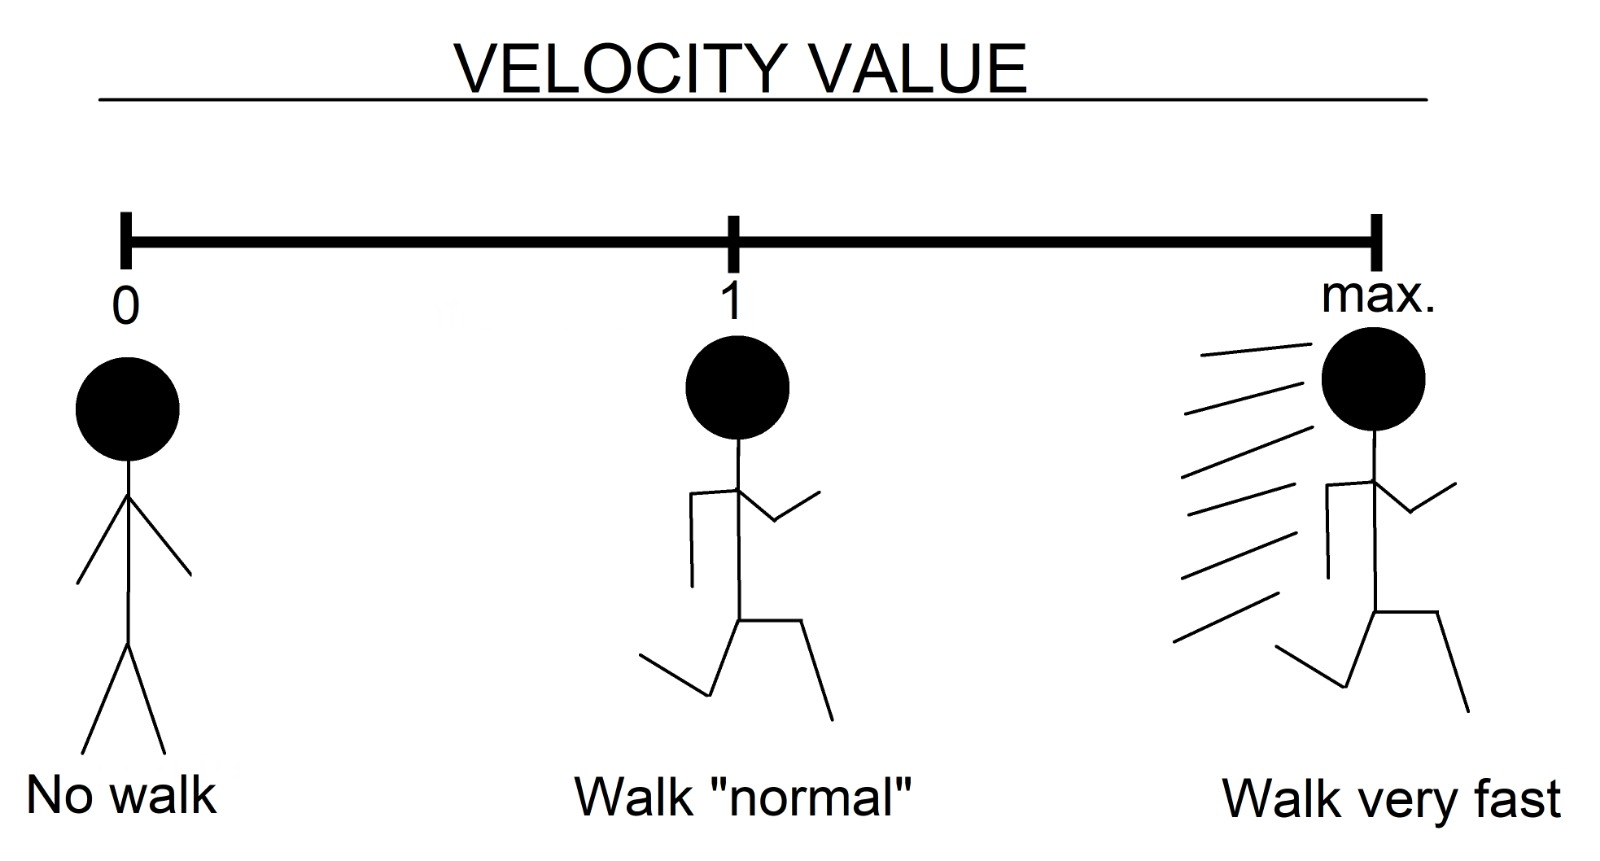
\includegraphics[width=1\textwidth]{figures/cap_4/velocity_value.jpeg}
  \caption{Esquema de parametrización de la velocidad}
  \label{fig:vel_value}
\end{figure}

Para conseguir este efecto, ha sido necesario dividir el tiempo de cada fotograma entre el parámetro de velocidad introducido, de esta manera, se consigue que cuando el parámetro sea menor que 1, el tiempo aumente, y lo contrario en caso de que el parámetro sea mayor que 1. Así también nos aseguramos de que el parámetro quede ``predeterminado'' si le pasamos velocidad igual a 1.

Sin embargo, se debe tener precaución a la hora de pasar este parámetro, ya que una velocidad demasiado baja hará que los fotogramas no vayan con la fluidez mínima requerida y el robot se mueva de manera poco realista, dejando demasiado espacio temporal entre un fotograma y el siguiente. De forma análoga, una velocidad demasiado alta provocará inestabilidad absoluta en la caminata, y los fotogramas siguientes ``atropellarán'' a los anteriores, haciendo que el robot caiga.

Para evitar que el usuario utilice valores inadecuados, cada una de estas funciones cuenta con un valor mínimo y uno máximo permitidos. Estos límites se especificarán en la explicación correspondiente de cada función, presentada más adelante.

Esta velocidad puede ser lineal, angular o lateral y tomar valores positivos y negativos, siguiendo estas normas:
\begin{itemize}
    \item \textit{Velocidad positiva}: Implica movimientos hacia adelante o a la derecha, dependiendo de si la velocidad es lineal o angular/lateral, respectivamente.
    \item \textit{Velocidad negativa}: Implica movimientos hacia atrás o la izquierda, dependiendo de si la velocidad es lineal o angular/lateral, respectivamente.
\end{itemize}

Este efecto se logra gracias a que hay patrones para ambas direcciones, y dependiendo del caso se utiliza uno u otro.

Cabe destacar que no sólo se ha parametrizado la velocidad, también se ha parametrizado el número de pasos que el robot puede dar. Este mínimo viene dado por el patrón predeterminado en formato CSV y puede ser 10 o 2, dependiendo del caso. Para parametrizarlo, simplemente se repite en un bucle \textit{for} el patrón \texttt{pasos\_indicados/mínimo} veces, por lo que el parámetro de los pasos también debe ser múltiplo del mínimo. Dicho valor mínimo también se detallará a continuación.

Cada una de estas funciones son como la mostrada en la \autoref{lst:funcion_rclpy}, debido a que estos patrones se logran mediante nodos ROS2 que deben ser invocados.

Estas funciones son las siguientes:
\begin{itemize}
    \item \textit{setL}: Esta función tiene como objetivo que NAO se desplace lateralmente (utilizando velocidad lateral). Los patrones utilizados se han recogido de webots y tiene un mínimo de 2 pasos, con velocidad mínima de -0.35 ó 0.35, dependiendo de la dirección a la que se quiera avanzar y una máxima de 4.35 ó -4.35. A continuación se adjunta un enlace\footnote{\url{https://youtu.be/I7xlrR8_ZJk}} a su vídeo demostrativo.
    \item \textit{setV}: Esta función se encarga de hacer al robot caminar en linea recta (utilizando velocidad lineal). El mínimo de pasos en este caso es algo especial, ya que, si se le pasa velocidad negativa, el patrón sólo tiene 2 pasos, por lo que en este caso, el bucle se repite \textit{5*pasos\_indicados}, para que el número de pasos aplique a ambos patrones, ya que el patrón de caminata hacia adelante tiene un mínimo de 10 y así ambos lo comparten. Ambos fueron recogidos de webots y los máximos y mínimos de velocidad son los mismos que para la función setL. Se puede apreciar su funcionamiento en este enlace\footnote{\url{https://youtu.be/bpGAtWTDSik}}.
    \item \textit{turnVel}: Esta función sirve para que el robot sea capaz de girar en el sitio con velocidad angular parametrizada. Ambos patrones utilizados son recogidos de webots, tienen un mínimo de 2 pasos y unas velocidades de 0.35 y -0.35 para el mínimo, y 1.9 y -1.9 para el máximo. Su vídeo demostrativo se encuentra en el siguiente enlace\footnote{\url{https://youtu.be/NH_6tGjlq7U}}.
    \item \textit{setW}: Esta función se encarga de mover a NAO describiendo una trayectoria de arco, a una velocidad lineal (V) fija por defecto, sus parámetros son los mismos que la función anterior. Los patrones utilizados fueron creados a base de editar el patrón CSV de la caminata hacia adelante. Puede apreciarse su funcionamiento en el siguiente vídeo\footnote{\url{https://youtu.be/X8-WW8bdEck}}.
    \item \textit{setNW}: Esta función es igual que la anterior, pero los arcos descritos son hacia atrás. Los patrones utilizados fueron creados a base de editar el patrón CSV de la caminata hacia atrás. No se adjunta vídeo de esta función por ser tan parecida a la anterior.
\end{itemize}

Pero, estas funciones por sí solas no representan una forma intuitiva de hacer que el robot camine, por lo que es necesaria una sexta función que encapsule todas estas (excepto la de setL, ya que esa es un modo de caminar más específico y se deja fuera) en una sola con una interfaz amigable para el usuario. Esta es la función \textit{setArc}, que recibe todos los parámetros necesarios para cada función explicada anteriormente (número de pasos, velocidad V o W, y el parámetro opcional \textit{printable}) para después llamarlas en función de los parámetros recibidos.

Para facilitar la comprensión de esta función, se incluye un esquema que muestra su impacto en la trayectoria del NAO en la \autoref{fig:setarc_esq}.

\begin{figure}[H]
  \centering
  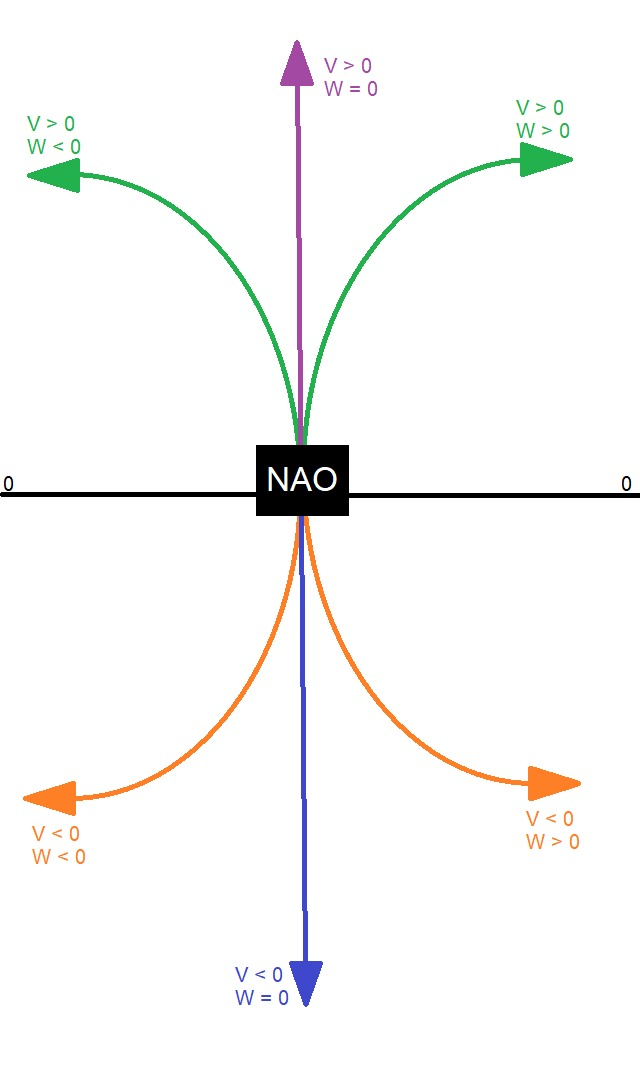
\includegraphics[height=0.8\textwidth]{figures/cap_4/esquema_movs.jpeg}
  \caption{Esquema de funcionamiento de la función \textit{setArc}}
  \label{fig:setarc_esq}
\end{figure}

El código de esta función tan importante y sencilla al mismo tiempo se encuentra en el \autoref{lst:setarc}
\begin{lstlisting}[language=Python, caption={Función setArc}, label={lst:setarc}, numbers=left, backgroundcolor=\color{gray!10}]    
def setArc(v,w,steps = 10):
    if (not ((0.35 <= abs(w) <= 1.9) or abs(w) == 0) or not (2 <= steps) or (steps%2 != 0)) or (not ((0.35 <= abs(v) <= 4.35) or abs(v) == 0) or not (10 <= steps) or (steps%10 != 0)):
        print("[setArc]: ERROR: La velocidad lineal debe estar entre +-0.35 y +-4.35 y la angular entre +-0.35 y +-1.9, y los pasos deben ser multiplos de 10")
        sys.exit(1)

    if v != 0 and w == 0:
        setV(v, steps, False)

    elif v != 0 and  w != 0:
        if v > 0: 
            setW(w, steps, False)
        else:
            setNW(w, steps, False)
    
    elif v == 0 and w != 0:
        turnVel(w, steps, False)
    
    elif v == 0 and w == 0:
        stand_still(False)

    else:
        print("[setArc] ERROR: Patron de movimiento no valido")
        sys.exit(1)
    
    print("[setArc]: Pasos completados")
\end{lstlisting}

\subsection{Funciones que utilizan sensores} \label{subsec:sensores}

También se han incluido en la biblioteca funciones cuya misión es leer los datos sensoriales y brindar información al respecto. Este es el caso de las funciones \textit{Read\_IMU} y \textit{get\_face}.

La primera de las funciones se encarga de devolver la aceleración en z que está experimentando el robot, para que después \textit{get\_face} la recoja y nos indique, en el caso de caída, si NAO está de \textit{cubito supino} (boca arriba), \textit{cubito prono} (boca abajo) o en una posición indeterminada.

Esto sirve para saber por ejemplo a qué patrón fijo de levantarse debemos llamar.

En el caso de la cámara, no se ha implementado una función concreta para utlizarla, se hablará de esto en el Capítulo \ref{cap:conclusiones}. 

En el siguiente enlace\footnote{\url{https://youtu.be/xJUYh2QJNuk}} se adjunta un vídeo demostrativo de estas funciones, aunque solo se ve \textit{get\_face}, porque usa \textit{Read\_IMU} para funcionar.

\section{Aplicación de ejemplo con el humanoide} \label{sec:aplicacion}

Esta aplicación, además de utilizar al NAO como robot de servicio, demuestra que la librería creada funciona correctamente. Esto es porque se ha desarrollado íntegramente utilizando sus funciones.

La aplicación consiste en que NAO transporte una caja hecha a medida para él, ya que su tamaño no permite otra alternativa. Como el modelo utilizado no tiene dedos, fue necesario adaptar la caja para que pudiera sostenerla de forma segura. El objetivo es moverla desde una mesa azul hasta una mesa naranja, ambas ajustadas a la escala del robot y ubicadas dentro de un invernadero. Por esta razón, la aplicación ha sido llamada \textit{GreenNao}.

El escenario utilizado ha sido íntegramente creado dentro de este Trabajo Fin de Grado, con ayuda de \textit{assets opensource} de Blender\footnote{\url{https://www.blender.org/}}. Este mundo también está en formato SDF (\cite{tutorial_mallas},\cite{parametros_fisicos_gazebo}) y se muestra en la \autoref{fig:mundo_invernadero}.

\begin{figure}[H]
  \centering
  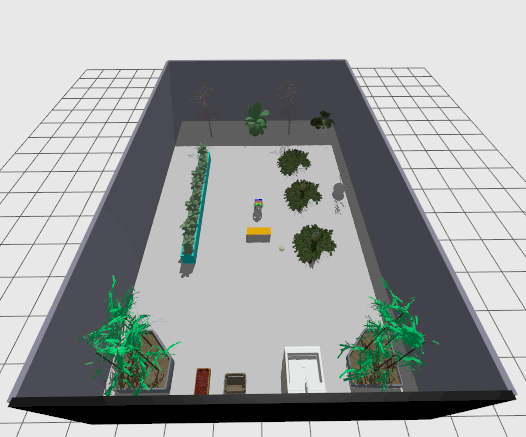
\includegraphics[width=1\textwidth]{figures/cap_4/mundo_invernadero.png}
  \caption{Mundo Invernadero para la aplicación de ejemplo}
  \label{fig:mundo_invernadero}
\end{figure}

Para llevar a cabo esta aplicación, simplemente se ha ido llamando a las funciones necesarias de la librería \texttt{CoordMovesLib} hasta conseguir el resultado esperado.

A continuación, en el \autoref{lst:aplicación} se muestra el código fuente de esta aplicación para demostrar el uso de funciones de la librería y se adjunta un vídeo\footnote{\url{https://youtu.be/obWjmRzKRCQ}} demostrativo de la misma, además de un par de  fotos en la \autoref{fig:aplicacion_1} y también en la \autoref{fig:aplicacion_2} para que se pueda apreciar mejor el montaje de esta aplicación de ejemplo.

\begin{lstlisting}[language=Python, caption={Aplicación GreenNao}, label={lst:aplicación}, numbers=left, backgroundcolor=\color{gray!10}]
import CoordMovesLib
import time

time.sleep(5)
CoordMovesLib.grab_box()
time.sleep(3)

for i in range(3):
  CoordMovesLib.turn("L", 60)

CoordMovesLib.turn("L", 40)

CoordMovesLib.setArc(1, 0)
time.sleep(3)

CoordMovesLib.release_box()
print("Terminado")
\end{lstlisting}

\begin{figure}[H]
  \centering
  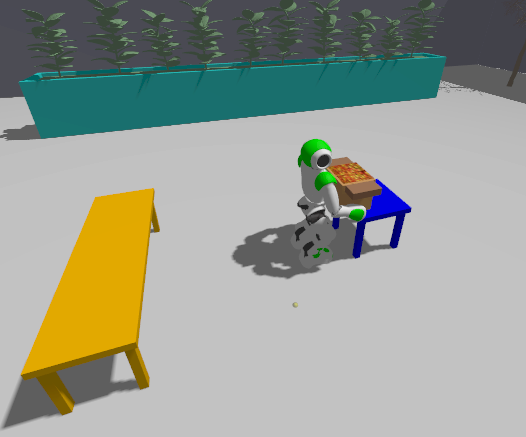
\includegraphics[width=0.7\textwidth]{figures/cap_4/app_1.png}
  \caption{Aplicación GreenNao. Vista lateral}
  \label{fig:aplicacion_1}
\end{figure}

\begin{figure}[H]
  \centering
  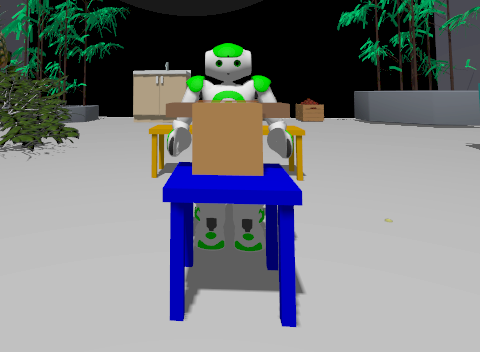
\includegraphics[width=0.7\textwidth]{figures/cap_4/app_2.png}
  \caption{Aplicación GreenNao. Vista frontal}
  \label{fig:aplicacion_2}
\end{figure}